
\noindent\begin{minipage}{\textwidth}
    \begin{table}[H]
        \centering
        \caption{Hiperparâmetros e Resultados do Melhor Modelo - efficientnet\_v10\_BR\_opt\_aug}
        \vspace{0.2cm}
        \resizebox{\textwidth}{!}{%
            \begin{tabular}{ll | lrrr}
                \hline
                \multicolumn{2}{c|}{\textbf{Hiperparâmetros}} & \multicolumn{4}{c}{\textbf{Métricas por Classe}} \\ \hline
                \textbf{Parâmetro} & \textbf{Valor} & \textbf{Classe} & \textbf{Precisão} & \textbf{Recall} & \textbf{F1-Score} \\ \hline
    Agendador (Patience) & 8 & 31.2 & 0,7124 & 0,7252 & 0,7188 \\ 
Agendador de LR & ReduceLROnPlateau & 31.3 & 0,5407 & 0,6011 & 0,5693 \\ 
Architecture & efficientnet\_b2 & 31.4 & 0,5219 & 0,6272 & 0,5697 \\ 
Batch Size & 32 & 32.3 & 0,8163 & 0,6349 & 0,7143 \\ 
Data Augmentation & False & 32.4 & 0,6429 & 0,5000 & 0,5625 \\ 
Decaimento de Peso (WD) & 0,0000 & 33.3 & 0,7179 & 0,6481 & 0,6813 \\ 
Dropout & 0,4926 & 41.4 & 0,4884 & 0,4468 & 0,4667 \\ 
Função de Perda & CrossEntropyLoss & 41.5 & 0,6596 & 0,7209 & 0,6889 \\ 
Hidden Units & 256 & 42.4 & 0,6102 & 0,5902 & 0,6000 \\ 
Label Smoothing & 0,1000 & 44.4 & 0,8529 & 0,9062 & 0,8788 \\ 
\cline{3-6} 
Otimizador & AdamW & \textbf{Média (Macro)} & 0,6798 & 0,6304 & 0,6464 \\ 
Taxa de Aprendizado (LR) & 7,01e-04 & \textbf{MCC} & \multicolumn{3}{c}{0,6006} \\ 
Unfreeze Layers & 7 &  & & &  \\ 
            \hline
            \end{tabular}%
        }
    \end{table}

    \begin{figure}[H]
        \centering
        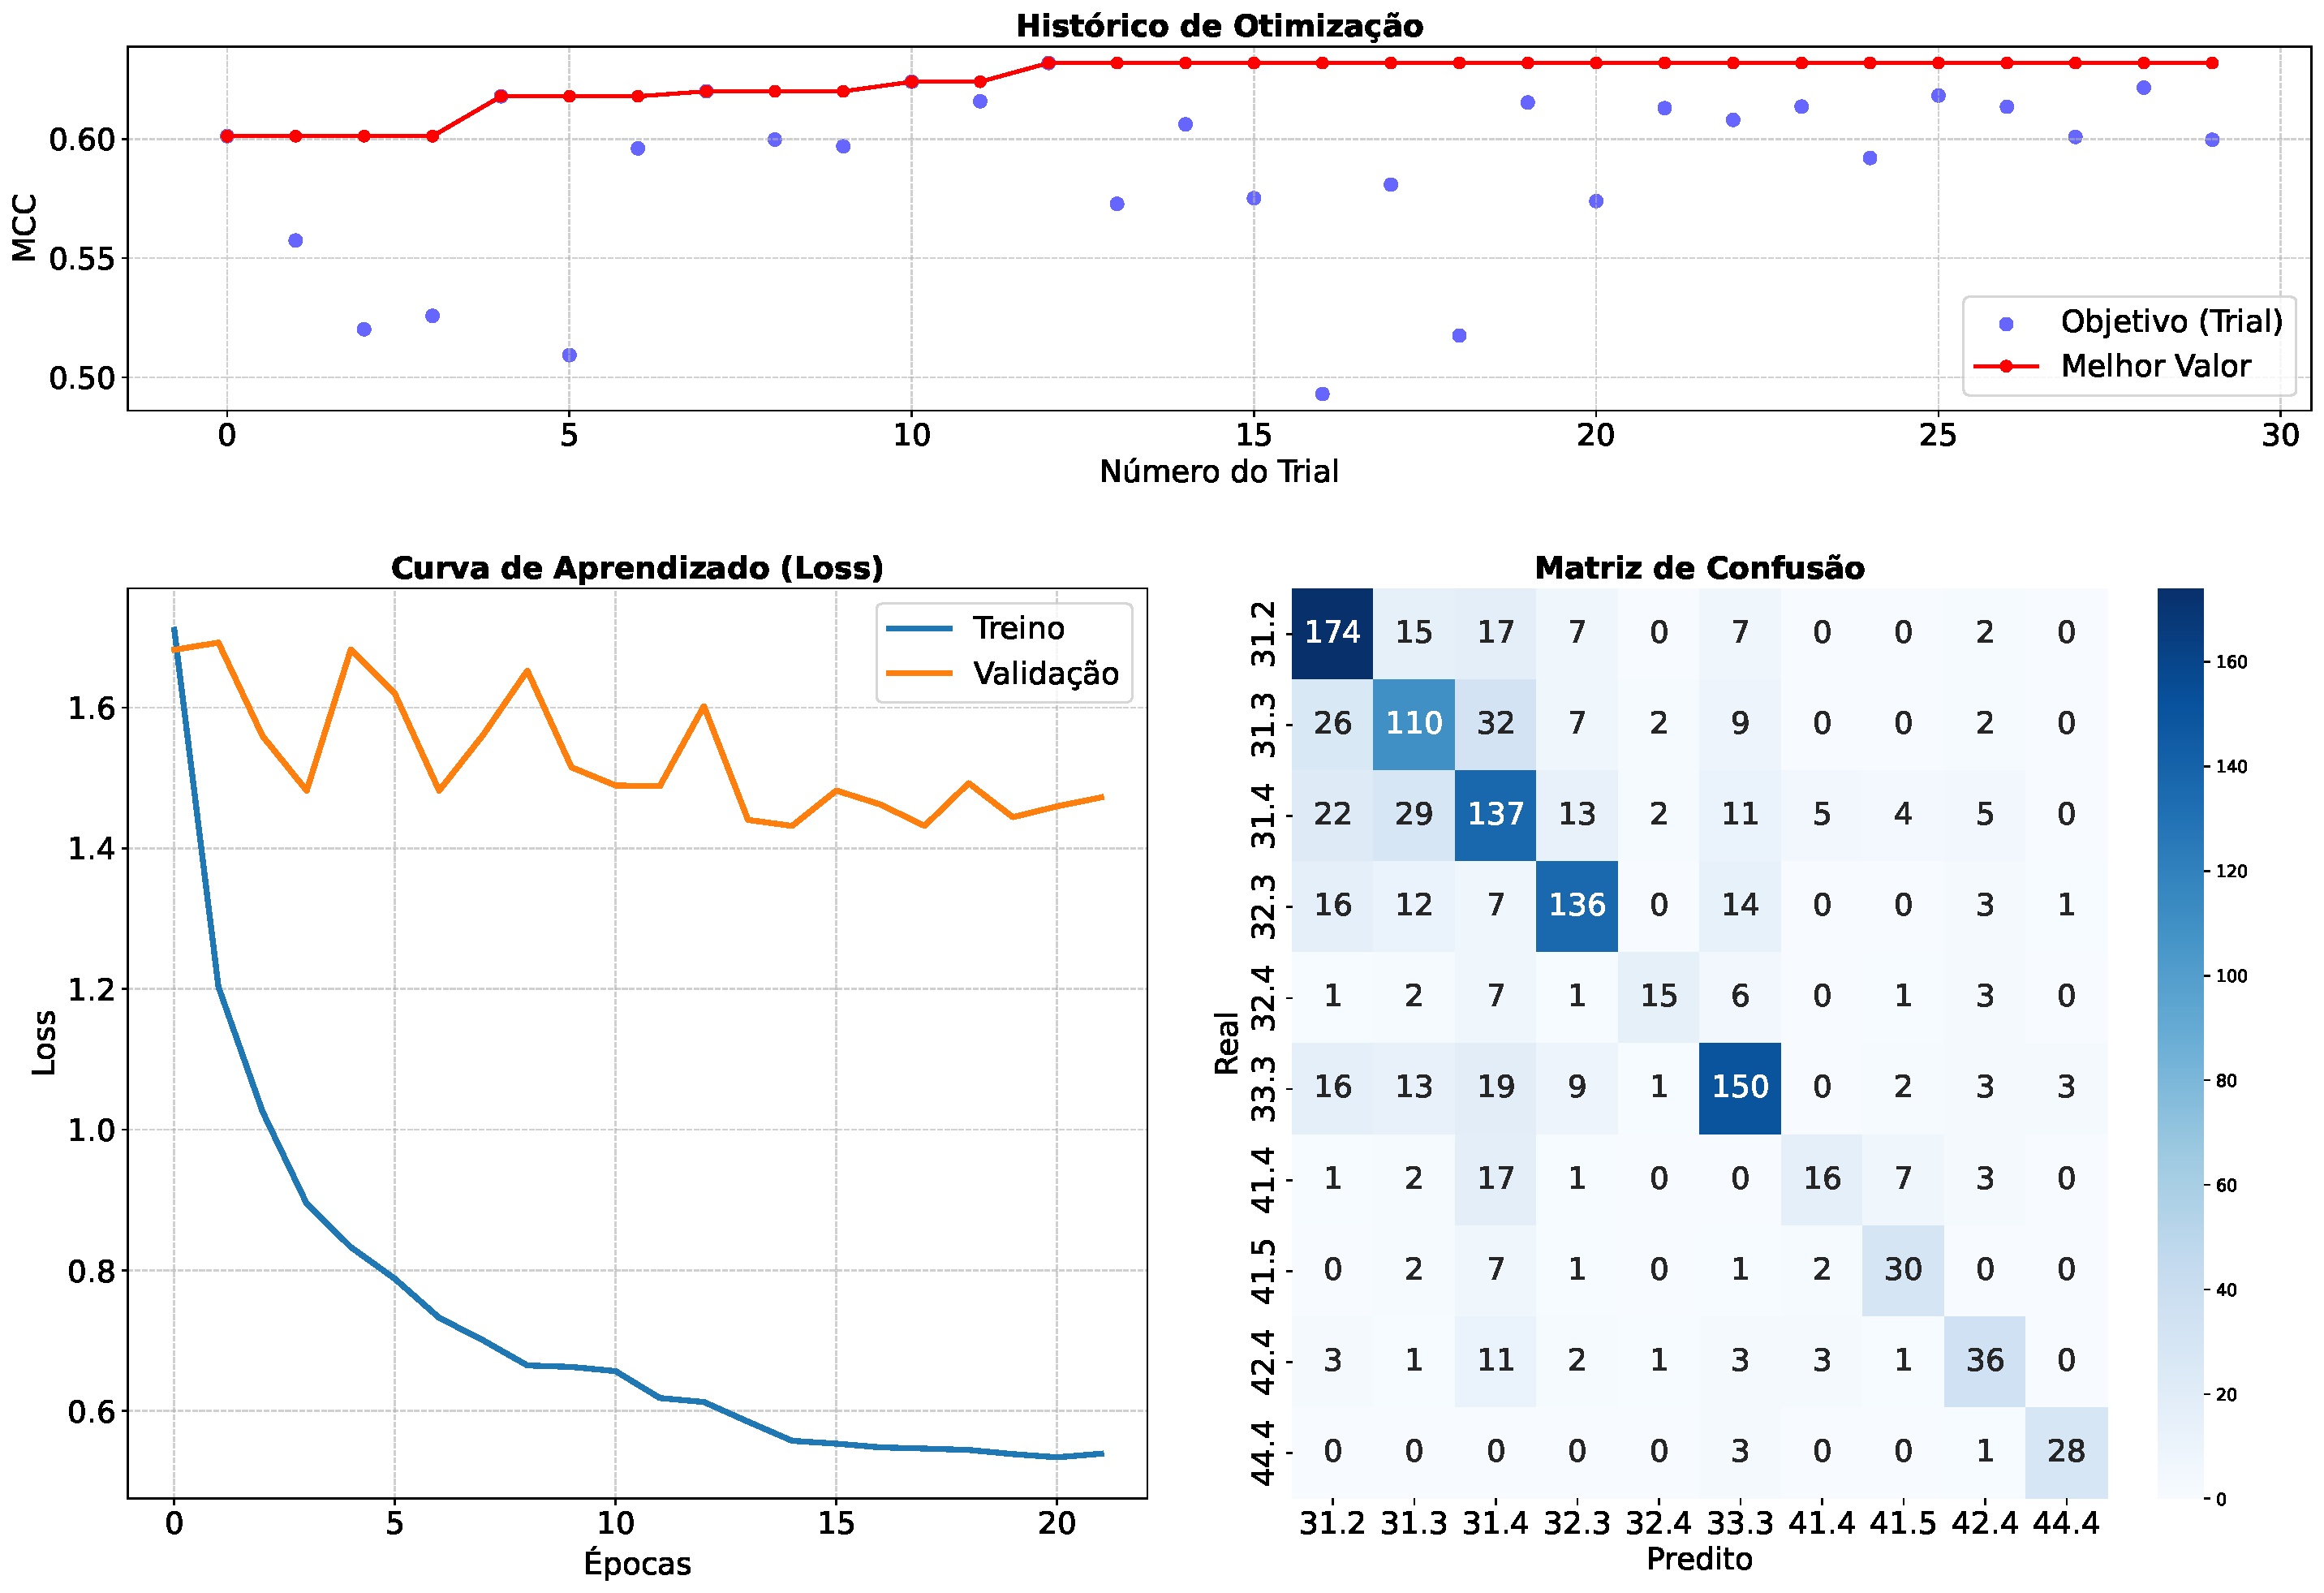
\includegraphics[width=0.85\textwidth]{tex/appendix/experiments/efficientnet_v10_BR_opt_aug/dashboard_consolidado.pdf}
        \caption{Histórico de Otimização, Curvas de Aprendizado e Matriz de Confusão - efficientnet\_v10\_BR\_opt\_aug}
    \end{figure}
\end{minipage}
\clearpage
